\chapter{State of Art}

Several methods have been developed in order to have a better speech enhancement. The state of art will be divided in two groups of algorithms: single channel and multiple channel. It is important to note that this algorithms can be mixed to obtain different kinds of noise reduction methods.

\section{Single Channel Algorithms}

\subsection{Voiced Activity Detection (VAD)}

Many methods of speech enhancement use the VAD method to make a difference between silence and speech periods. This periods are always differentiated by each of the STFT frames processed. The voiced sounds are periodic and usually have more energy that unvoiced sounds, also, unvoiced sounds are more noise-like and have more energy than silence segments.

The VAD can be used in many implementations as speech recognition, voice compression, noise estimation and suppression, and echo cancellation. For this, some methods have been developed. 
Probably the simplest VAD is Energy Level Detection \cite{Faneuff2002SpatialCar}, in which the initial noise spectrum, mean, and variance are calculated assuming the initial frames are only noise. After this, the thresholds are calculated for speech and noise decisions and all statistics are gradually updated when a noise frame is detected. The process diagram can be seen in figure \ref{fig:VADener}.

\begin{figure}[!ht]
  \center
	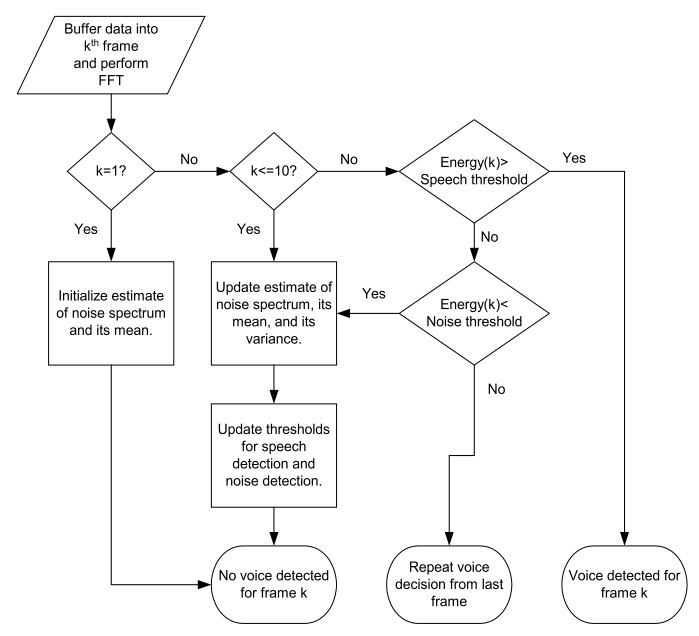
\includegraphics[width=110mm]{State_of_Art/VADener}
	\caption{VAD with energy detection\cite{Faneuff2002SpatialCar}.}
	\label{fig:VADener}
\end{figure}

Some other methods can be found in \cite{Faneuff2002SpatialCar}, \cite{Rubio2007Two-microphoneEstimates},\cite{Rosca2002MultichannelEnvironments}, \cite{Gerkmann2011NoisePresence},\cite{Nelke2013DualProbability}. Some of them are listed:

\begin{itemize}
\item Zero crossing rates: these can be calculated for each frame and compared with a threshold. The zero crossing rate of noise is assumed to be considerably larger than the one of speech. This assumption works well at high SNR values, but has problems at low SNR and in the presence of periodic noise.

\item Periodicity: The detector uses a least-squares periodicity estimator, LSPE, on the input signal and triggers when a significant amount of periodicity is found.


\item Speech Presence Probability (SPP):  it is shown \cite{Gerkmann2011NoisePresence} that it is possible to create a limited maximum likelihood estimator, then use it for the estimation of the a priori signal-to-noise ratio (SNR), and this resulting noise power estimate can be updated when the a posteriori SNR is below a certain threshold and, finally, this threshold can be seen as a voice activity detector. 


\end{itemize}

\subsection{Spectral subtraction}

This algorithm uses the short-term spectral magnitude of the noisy speech and estimate or reference of the noise signal. Most of the single channel spectral subtraction methods use a VAD to determine if there is silence or not in order to get an accurate noise estimate and the noise is assumed to be short term stationary so that noise from silence frames can be used to remove noise from voiced frames as shown in figure \ref{fig:duagSS}.


\begin{figure}[!ht]
  \center
	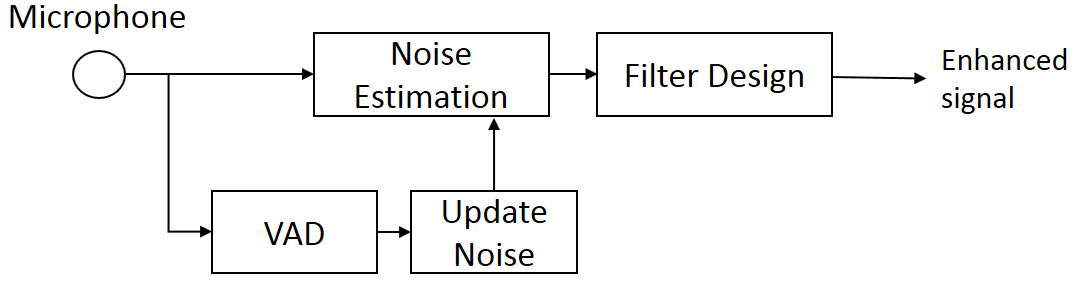
\includegraphics[width=110mm]{State_of_Art/duagSS}
	\caption{Basic Spectral Subtraction.}
	\label{fig:duagSS}
\end{figure}


Many articles show different ways of using the spectral subtraction as \cite{Ephraim1984SpeechEstimator}, \cite{MeyerSubtraction.pdf}, \cite{Smaragdis1998BlindDomain}, \cite{Abdelaziz2005Real-TimeEnhancement}.

The spectral subtraction always uses a VAD. This is used to know the noise power only in the silence periods and this information is used to erase the noise from the speech as we can see in the figure \ref{fig:scspecSubs}.

\begin{figure}[!ht]
  \center
	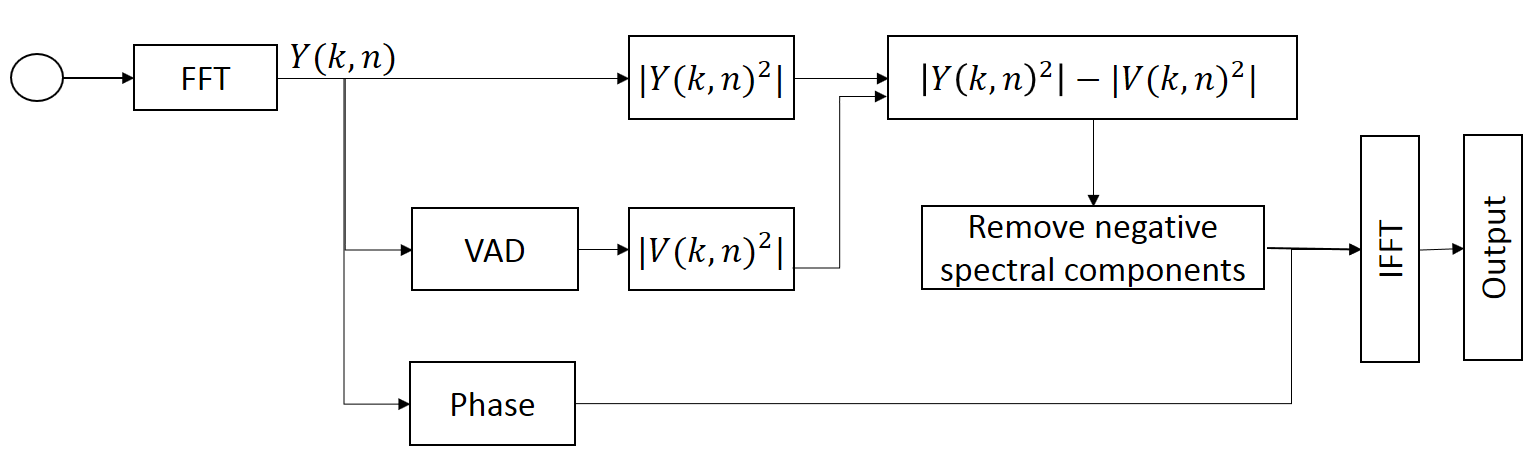
\includegraphics[width=110mm]{State_of_Art/scspecSubs}
	\caption{Single Channel Spectral Subtraction.}
	\label{fig:scspecSubs}
\end{figure}


\subsection{Talker isolation}

It is necessary to isolate the desired speech from other speech sources and noise. In this case, separating the sources is crucial since the desired and undesired speech have similar spectra and comparable amplitudes.

It is used the frequency and amplitude continuity to track the desired talker. Binaural spatial cues are used to discriminate pitch frequencies that are too close to resolve spectrally. In \cite{Luo1994AReverberation} they show an example using a combination of techniques for advanced pitch tracking and talker isolation, it is used frequency and amplitude continuity to track the desired talker.



\section{Multiple Channel Algorithms}


\subsection{Sources separation}

The separation of sources is an approach in which the source signals are estimated from the mixed signals observed in each channel. This technique is used in sound systems in order to erase noise or to erase the cross-talking in communications. This system can be modeled as seen in figure \ref{fig:sepa} (with 2 sources).


\begin{figure}[!ht]
  \center
	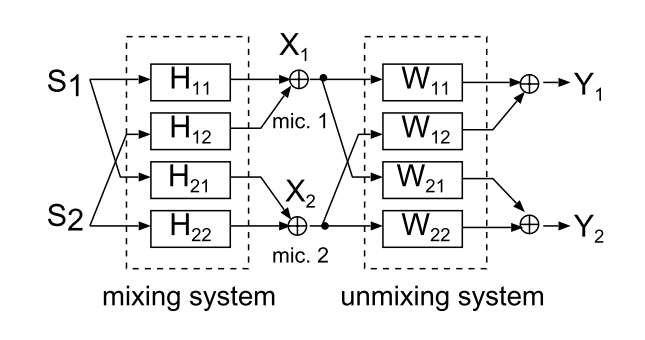
\includegraphics[width=90mm]{State_of_Art/sepa}
	\caption{Separation of sources system configuration.}
	\label{fig:sepa}
\end{figure}

Many methods have been developed to achieve a proper separation of sources. In \cite{Smaragdis1998BlindDomain} it is shown a method in which, as some other methods like \cite{Bourgeois2004Frequency-domainCorrelation} and \cite{Mei2006BlindCriterion}, every filter of the unmixing system ($W_{ij}$) is found by an estimation of the mixing system ($H_{ij}$). 



\subsection{Beamforming}

Beamforming is the term used for steering an array of sensors (microphones) to have unity gain in the direction of the desired source and attenuate the signals with origin in other directions. Source localization can be important to improve the effect of beamforming \cite{Faneuff2002SpatialCar}. This can be used as a noise reduction method due to it's capacity of localization, that means that the noise (which comes from different directions than the voice) will be attenuated. 


The technique of beamforming is used to capture multiple sound inputs $s(t)$ in the farfield and, after filtering and addition obtain a reference signal $Z$ \cite{Faneuff2002SpatialCar}. 


%\begin{figure}[!ht]
%  \center
%	\includegraphics[width=110mm]%{Kap3/bf_beam_pattern}
%	\caption{Beamforming system %configuration.}
%	\label{fig:bf_beam_pattern}
%\end{figure}


One technique called the "delay and sum beamformer" , which is probably the simplest, consist in apply a phase delay to the input signals to steer the main lobe directivity to an specific direction. 

\subsection{Coherence and Speech Presence Probability}

In \cite{Nelke2013DualProbability} is proposed one noise estimation method based in the speech presence probability value showed in \cite{Gerkmann2011NoisePresence} and the coherence function, which behaves as a measure of spectral similarity between signals. The coherence function, due to the noise characteristics of noise in diffuse field, has low values for noisy segments and a high value for speech segments.

\subsection{Multi-Channel Wiener Filter}

The Wiener filter is a filter used to produce an estimate of a desired or target, assuming known stationary signal and noise spectra, and additive noise. The goal of the this filter is to find a statistical estimate of an unknown signal using a reference signal as an input and filtering this signal to produce the estimate as an output. 
In \cite{Yong2013} it is proposed a multichannel method which also uses one single channel method as reference. This algorithm will be described in detail later since it was chosen for implementation.


